\section{Monday for MAT4002}\index{Monday_lecture}
\subsection{Quotient Topology}
Now given a topologcal space $X$ and an equivalence relation $\sim$ on it, our goal is to construct a topology on the space $X/\sim$.
\begin{proposition}\label{pro:6:1}
Suppose $(X,\mathcal{T})$ is a topological space, and $\sim$ is an equivalene relation on $X$.
Define the canonical projection map:
\[
\begin{array}{ll}
p:&X\to X/\sim\\
\text{with}&x\to[x]
\end{array},
\]
which assigns each point $x\in X$ into the equivalence class $[x]$.
Then define a family of subsets $\tilde{\mathcal{T}}$ on $X/\sim$ by:
\[
\tilde{U}\subseteq X/\sim
\text{ is in $\tilde{\mathcal{T}}$ if }
p^{-1}(\tilde{U})
\text{ is in $\mathcal{T}$}
\]
Then $\tilde{\mathcal{T}}$ is a topology for $X/\sim$, called the \emph{quotient topology}, and $(X/\sim,\tilde{\mathcal{T}})$ is called the quotient space,
and $p:X\to X/\sim$ is called the \emph{natural map}.
\end{proposition}

\begin{proof}
\begin{enumerate}
\item
$p^{-1}(X/\sim) =X\in\mathcal{T}$ and $p^{-1}(\emptyset) = \emptyset\in\mathcal{T}$, which implies 
$X/\sim\in\tilde{\mathcal{T}}$ and $\emptyset\in\tilde{\mathcal{T}}$.
\item
Suppose that $\tilde{U},\tilde{V}\in\tilde{\mathcal{T}}$, then we imply
\[
p^{-1}(\tilde{U}),p^{-1}(\tilde{V})\in\mathcal{T}
\implies
p^{-1}(\tilde{U}\cap\tilde{V})\in\mathcal{T},
\]
i.e., $\tilde{U}\cap\tilde{V}\in\tilde{\mathcal{T}}$.
\item
Following the similar argument in (2), and the relation
\[
p^{-1}\left(\bigcup\tilde{U}_i\right)=\bigcup p^{-1}(\tilde{U}_i),
\]
we conclude that $\tilde{T}$ is closed under countably union.
\end{enumerate}
The proof is complete.
\end{proof}
\begin{remark}
\begin{enumerate}
\item
The proposition~(\ref{pro:6:1}) claims that $\tilde{U}$ is open in $X/\sim$ iff $p^{-1}(\tilde{U})$ is open in $X$.
The general question is that, does $p(U)$ is open in $X/\sim$, given that $U$ is open in $X$?
This may not necessarily hold. (See example~(\ref{exp:6:4}))
In general $p^{-1}(p(U))$ is strictly larger than $U$, and may not be necessarily open in $X$, even when $U$ is open.
\item
By definition, we can show that $p$ is continuous.
\end{enumerate}
\end{remark}

To fill the gap on the question shown in the remark, we consider the notion of the open mapping:
\begin{definition}[Open Mapping]
A function $f:X\to Y$ between two topological spaces is an \emph{open mapping} if for each open $U$ in $X$, $f(U)$ is open in $Y$.
\end{definition}
\begin{remark}
From the remark above, we can see that:
\begin{enumerate}
\item
Not every continuous mapping is an open mapping
\item
The canonical projection mapping $p$ is not necessarily be an open mapping.
\end{enumerate}
\end{remark}

\begin{example}\label{exp:6:4}
\begin{enumerate}
\item
The mapping $p:[0,1]\times[0,1]\to([0,1]\times[0,1])/\sim$ sending the square to the Mobius band $M$ is not an open mapping:

Consider the open ball $U=B_{1/2}((0,0))$ in $[0,1]\times[0,1]$.
Note that $p(U)$ is open in $M$ iff $p^{-1}(p(U))$ is open in $[0,1]\times[0,1]$.
We can calculate $p^{-1}(p(U))$ explicitly:
\[
p^{-1}(p(U)) = U\cup\{(1,y)\mid 1/2\le y\le 1\},
\]
which is not open.
\end{enumerate}
\end{example}

\subsection{Properties in quotient spaces}
\subsubsection{Closedness on $X/\sim$}
\begin{proposition}
A subset $\tilde{V}$ is closed in the quotient space $X/\sim$ iff $p^{1}(\tilde{V})$  is closed in $X$, where $p:X\to X/\sim$ denotes the canonical projection mapping.
\end{proposition}
\begin{proof}
It follows from the fact that
\[
p^{-1}\left((X/\sim)\setminus \tilde{V}\right)
=
X\setminus p^{-1}(\tilde{V})
\]
\end{proof}


\subsubsection{Isomorphism on $X/\sim$}
The quotient space can be used to study other type of spaces:

\begin{example}\label{exp:6:5}
Consider $X=[0,1]$. We define $x_1\sim x_2$ if:
\[
\begin{array}{lll}
x_1=0,x_2=1,
&
\text{or}
&
x_1=1,x_2=0
\end{array}
\]
In other words, the partition on $X$ is given by:
\[
X = \{0,1\}\cup(\bigcup_{x\in(0,1)}\{x\})
\]
The quotient space seems ``glue'' the endpoints of the interval $[0,1]$ together, shown in the figure below:
\begin{figure}[H]
\centering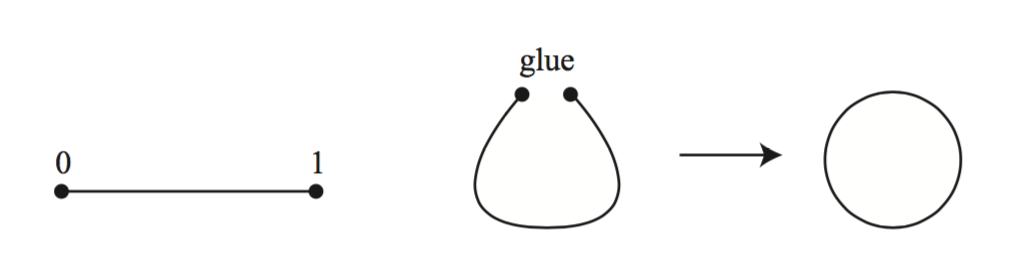
\includegraphics[width=0.6\textwidth]{week6/Fig_4}
\end{figure}
It is intuitive that the constructed quotient space should be homeomorphic to a circle $S^1$. We will give a formal proof on this fact.
\end{example}
\begin{proposition}\label{pro:6:3}
Let $X$ and $Z$ be topological spaces, and $\sim$ an equivalence relation on $X$.
Let $g:X/\sim\to Z$ be a function, and $p:X\to X/\sim$ is a projection mapping
The mapping $g$ is continuous if and only if $g\circ p:X\to Z$ is continuous.
\end{proposition}
\begin{proof}
\begin{enumerate}
\item
\textit{Necessity}.
Suppose that $g$ is continuous. It's clear that $p$ is continuos, i.e, $g\circ p:X\to Z$ is continuous.
\item
\textit{Sufficiency}.
Suppose that $g\circ p:X\to Z$ is continuous.
Given any open $U$ in $Z$, we imply $(g\circ p)^{-1}(U) = p^{-1}g^{-1}(U)$ is open in $X$.
By definition of the quotient topology, we imply $g^{-1}(U)$ is open in $X/\sim$.
Therefore, $g$ is continuous.
\end{enumerate}
\end{proof}
\begin{remark}
This useful lemma can be generalized into the case for generlized canonical projection mapping, called quotient mapping.
\begin{definition}[Quotient mapping]
A map $p:X\to Y$ between topological spaces is a \emph{quotient mapping} if
\begin{enumerate}
\item
$p$ is \emph{surjective}; and
\item
$p$ is continuous;
\item
For any $U\subseteq Y$ such that $p^{-1}(U)$ is open in $X$, we imply
$U$ is open in $Y$.
\end{enumerate}
\end{definition}
The canonical projection map is clearly a quotient map. Actually, a stronger version of proposition~(\ref{pro:6:3}) follows:
\begin{proposition}\label{pro:6:4}
Suppose that $p:X\to Y$ is a quotient map and that $g:Y\to Z$ is any mapping to another space $Z$.
Then $g$ is continuous iff $g\circ p$ is continuous.
\end{proposition}
\begin{proof}
The proof follows similarly as in proposition~(\ref{pro:6:3}).
\end{proof}
\end{remark}

Now we give a formal proof of the conclusion in the example~(\ref{exp:6:5}):
\begin{proof}
Define the mapping
\[
\begin{array}{ll}
f:&[0,1]\to S^1\\
\text{with}&t\mapsto(\cos2\pi t,\sin 2\pi t).
\end{array}
\]
Since $f(0)=f(1)$, the function $f$ induces a well-defined function
\[
\begin{array}{ll}
g:&[0,1]/\sim\to S^1\\
\text{with}&[t]\mapsto f(t)
\end{array}
\]
such that $f=g\circ p$, where $p$ denotes the canonical projection mapping.
Note that $f$ is continuous.
By proposition~(\ref{pro:6:3}), we imply $g$ is continuous.
Furthermore,
\begin{enumerate}
\item
Since $[0,1]$ is compact and $p$ is continuous, we imply $p([0,1])=[0,1]/\sim$ is compact
\item
$S^1$ is Hausdorff
\item
$g$ is a bijection
\end{enumerate}
By applying theorem(\ref{The:5:3}), we conclude that $g$ is a homeomorphism, i.e., $[0,1]/\sim$ and $S^1$ are homeomorphic.

\end{proof}
The argument in the proof can be generalized into the proposition below:
\begin{proposition}\label{pro:6:5}
Let $f:X\to Y$ be a surjective continuous mapping between topologcial spaces.
Let $\sim$ be the equivalence relation on $X$ defined by the partition $\{f^{-1}(y)\mid y\in Y\}$ (i.e., $f(x)=(x')$ iff $x\sim x'$).
If $X$ is compact and $Y$ is Hausdorff, then $X/\sim$ and $Y$ are homeomorphic.
\end{proposition}
\begin{remark}
The proposition~(\ref{pro:6:5}) is a pattern of argument we should use several times.
In order to show $X/\sim$ and $Y$ are homeomorphic, we should think up a surjective continuous mapping $f:X\to Y$ ``with respect to the identifications'', i.e., $f(x_1)= f(x_2)$ whenever $x_1\sim x_2$.
Therefore $f$ will induce a well-defined function $g:X/\sim\to Y$ such that $f = g\circ f$.
Then checking the conditions in theorem(\ref{The:5:3}) leads to the desired results.
\end{remark}

\paragraph{Torus}
We now study the torus in more detail.
\begin{enumerate}
\item
Consider $X=[0,1]\times[0,1]$ and define $(s_1,t_1)\sim(s_2,t_2)$ if one of the following holds:
\begin{itemize}
\item
$s_1=s_2$ and $t_1=t_2$;
\item
$\{s_1,s_2\}=\{0,1\}$, $t_1=t_2$;
\item
$\{t_1,t_2\}=\{0,1\}$ and $s_1=s_2$;
\item
$\{s_1,s_2\}=\{0,1\}$, $\{t_1,t_2\}=\{0,1\}$
\end{itemize}
The corresponding quotient space $([0,1]\times[0,1])/\sim$ is hoemomorhpic to the $2$-dimension torus $\mathbb{T}^2$.
\begin{proof}
Define the mapping $f:[0,1]\times[0,1]\to\mathbb{T}^2$ as $(t_1,t_2)\mapsto(e^{2\pi i t_1},e^{2\pi i t_2})$. 
\begin{enumerate}
\item
$f$ is surjective, which also implies $\mathbb{T}^2 = f([0,1]\times[0,1])$ is compact.
\item
$\mathbb{T}^2$ is Hausdorff
\item
It's clear that $(s_1,t_1)\sim(s_2,t_2)$ implies $f(s_1,t_1)=f(s_2,t_2)$. Conversely, suppose
\[
\begin{array}{ll}
e^{2\pi i s_1}=e^{2\pi i s_2},
&
e^{2\pi i t_1}=e^{2\pi i t_2}
\end{array}
\]
By the familiar property of $e^{ix}$, we imply either $t_1=t_2$ or $\{t_1,t_2\}=\{0,1\}$; and either $s_1=s_2$ or $\{s_1,s_2\}=\{0,1\}$
\end{enumerate}
By applying proposition~(\ref{pro:6:5}), we conclude that $([0,1]\times[0,1])/\sim$ is homeomorphic to $\mathbb{T}^2$.
\end{proof}
\item
Consider the closed disk $\mathbb{D}^2=\{(x,y)\in\mathbb{R}^2\mid x^2+y^2\le 1\}$,
and defube $(x_1,y_1)\sim(x_2,y_2)$ if one of the following holds:
\begin{itemize}
\item
$x_1=x_2$ and $y_1=y_2$;
\item
$(x_1,y_1)$ and $(x_2,y_2)$ are in the boundary circle $\mathbb{S}^1$
\end{itemize}
The corresponding quotient space $\mathbb{D}^2/\sim$ is hoemomorhpic to the $2$-dimension sphere $\mathbb{S}^2=\{(x,y,z)\mid x^2+y^2+z^2=1\}$.
\begin{proof}
Define the mapping
\[
\begin{array}{ll}
f:&\mathbb{D}^2\to\mathbb{S}^2\\
\text{with}&(0,0)\mapsto(0,0,1)\\
&(x,y)\mapsto\left(\frac{x}{\sqrt{x^2+y^2}}\sin(\pi\sqrt{x^2+y^2}), \frac{y}{\sqrt{x^2+y^2}}\sin(\pi\sqrt{x^2+y^2}), \cos(\pi\sqrt{x^2+y^2})\right)
\end{array}
\]
It's easy to check the conditions in proposition~(\ref{pro:6:5}), and we conclude that $\mathbb{D}^2/\sim$ is hoemomorhpic to $\mathbb{S}^2$
\end{proof}

\end{enumerate}











